\chapter{FaceItTools}
\section{Introduzione alla piattaforma}
\textit{FaceitTools.com} è una piattaforma di Larning Analytics sviluppata da studenti dell'Università di Padova che mette a disposizione dei corsi di varie materie universitarie strutturati principalmente in spidergram.
L'obiettivo è di facilitare l'apprendimento e mettere in evidenza come i corsi siano collegati tra loro e fornisce dei quiz sui quali si può essere valutati dai docenti.
\\Offre inoltre un sistema di raccolta feedback su domande d'esame archiviate in un database MongoDB che l’utente può cercare e filtrare usando una tabella Bootstrap.
\\Sulla base dei feedback viene effettuata un'analisi della difficoltà delle domande, infatti una volta inviate le risposte alle domande, viene visualizzato attraverso un grafico a barre il numero di risposte inviate e la difficoltà media percepita.
\\Questi feedback non sono utili sono agli studenti, ma anche ai docenti che possono capire se i corsi necessitano di essere rimodellati per essere più efficaci.
\begin{figure}[h]
    \centering
    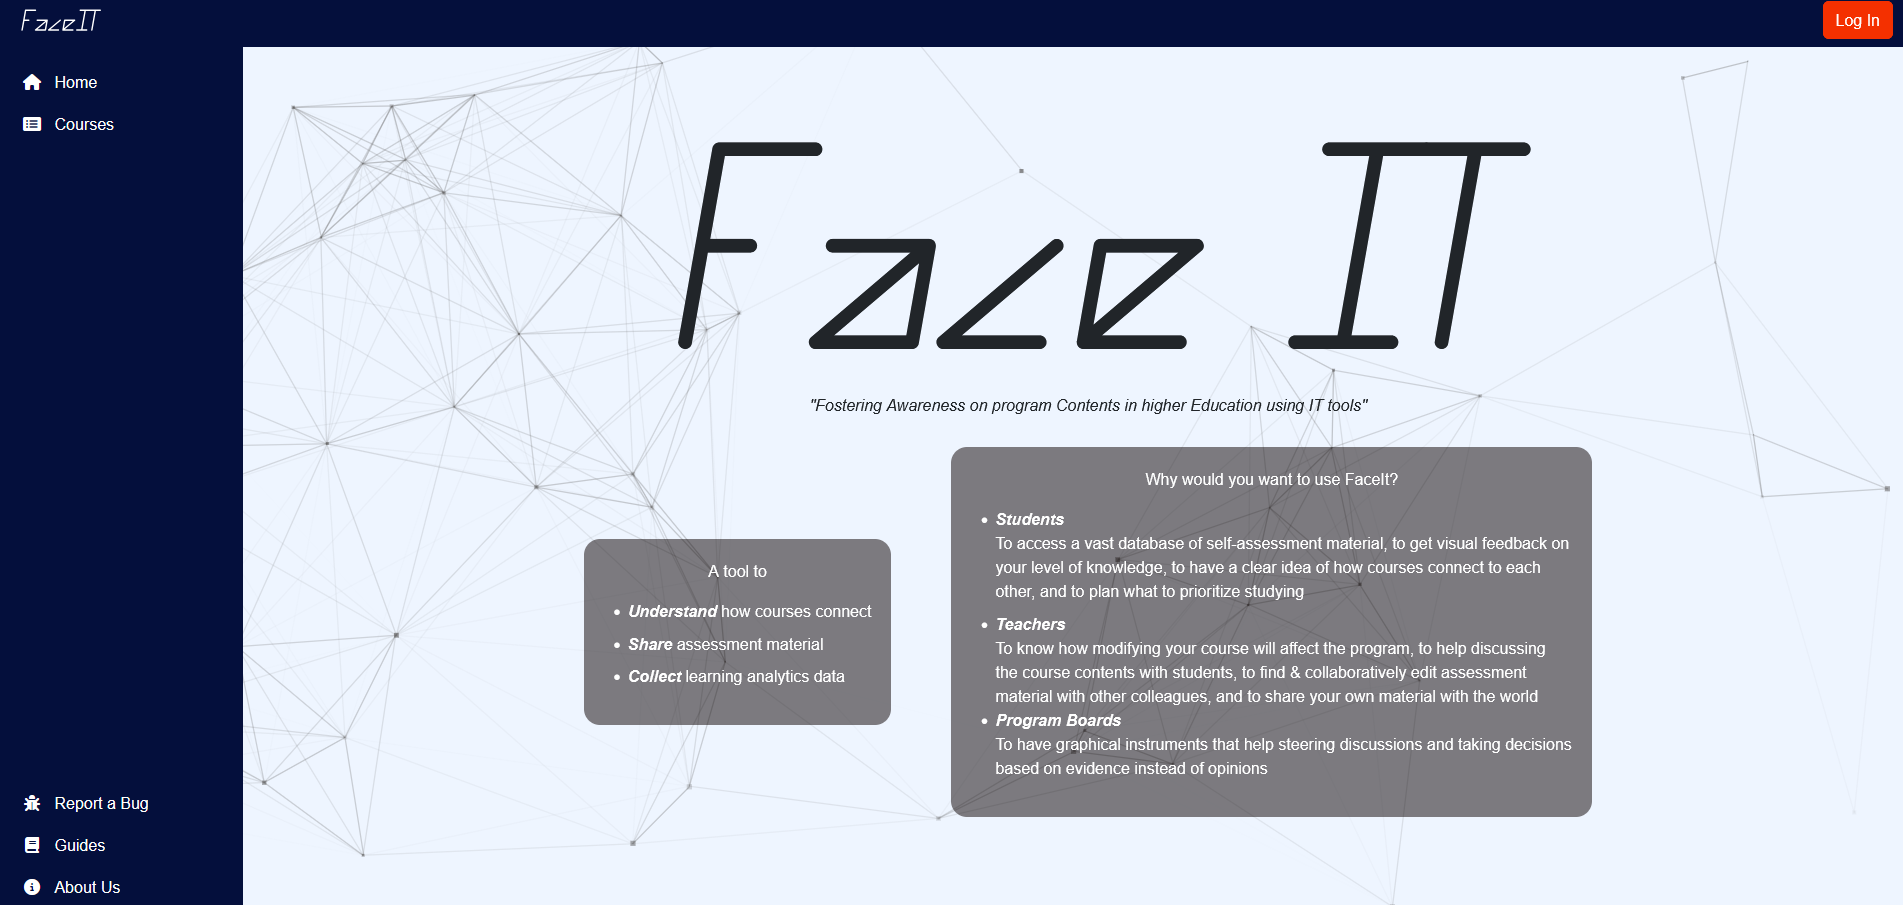
\includegraphics[width=0.65\textwidth]{Immagini/FaceItTools.PNG}
    \caption{FaceItTools homepage}
\end{figure}
\subsection{Ananlisi delle problematiche}
\subsection{Benefici di una trasformazione blockchain-oriented}
\section{Raccomandazioni per gli sviluppatori}